\section{OTA Designbeispiel}

\subsection{Spezifikationen}

Für die vorgegebenen Spezifikationen soll eine Schaltung entwickelt werden.

\vspace{-0.3cm}

\begingroup
\setlength{\columnseprule}{0pt}
\begin{multicols}{2}
    \begin{description}
        \item[Open Loop Gain] $a_\text{OL}$
        \item[Last] $C_\text{L}$
        \item[GBW]  
        \item[Phase Margin] $\Phi_\text{M}$
        \item[Stabilität] Unity gain stable or not
        \item[Slew Rate] SR
        \item[Versorgungsspannung] $V_\text{CC}$
        \item[Output Swing]
        \item[Offset Voltage] $V_\text{OS}$
    \end{description}
\end{multicols}
\endgroup



\subsection{Designablauf}

\begin{minipage}[t]{0.6\columnwidth}
    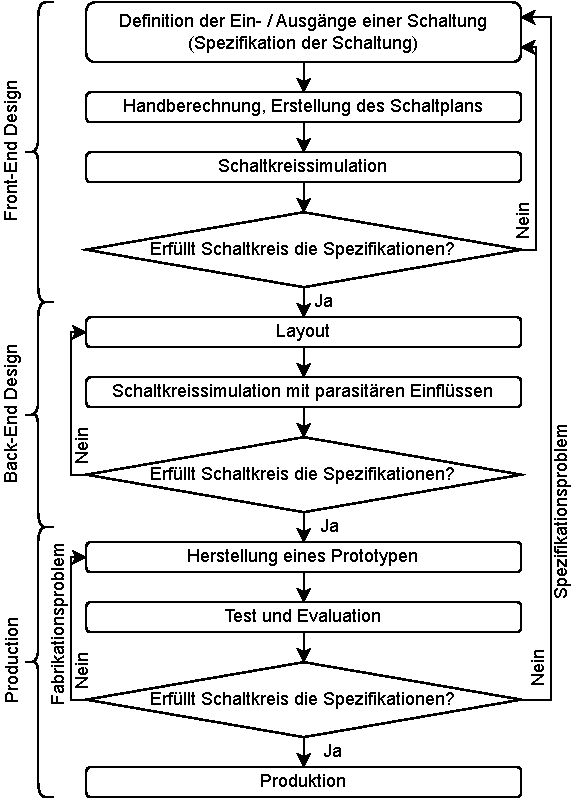
\includegraphics[width=\columnwidth, align=t]{images/12_OTA_design.pdf}
\end{minipage}
\hfill
\begin{minipage}[t]{0.38\columnwidth}   % NOTE: [Simi] @Flurin: So ganz zufrieden bin ich damit nicht... vielleicht sollten wir doch besser das Enum nehmen...
    \raggedright

    \paragraph{Front-End-Design}
    Der OTA ist typischerweise ein Sub-Block einer grösseren Schaltung.
    Es wird ein erster Schaltungsentwurf erstellt.
    Bei der Simulation können (mangels Layout) noch keine parasitären Effekte berücksichtigt werden.

    \medskip

    \paragraph{Back-End Design}
    Das Layout des OTAs wird gezeichnet. 
    Extraktion fügt der Netzliste parasitäre Komponenten zu, was eine sehr wirklichkeitsnache Simulation des Designs erlaubt.

    \medskip

    \paragraph{Production}
    Ev. wird OTA (allenfalls mit weiteren kritischen Komponenten) auf einem Prototyp integriert und evaluiert.
    Häufig wird auch die gesamte Schaltung als Prototyp realisiert. 

    \medskip

    \textbf{Hinweis:} Nur das Front-End Design ist Gegenstand dieser Vorlesung!
\end{minipage}



% \begin{enumerate}
%     \item Spezigikation: Definition der Ein- und Ausgänge einer Schaltung\label{enum:spec}
%     \item Handrechnungen, Erstellen eines Schaltplanes
%     \item Schaltkreissimulation
%     \item Spezifikationen erfüllt? Ja: gut. Nein: zurück zu Schritt~\ref{enum:spec}
%     \item Layout\label{enum:layout}
%     \item Schaltkreissimulation mit parasitären Einflüssen
%     \item Spezifikationen erfüllt? Ja: gut. Nein: zurück zu Schritt~\ref{enum:layout}
%     \item Herstellen eines Prototypen\label{enum:prototyp}
%     \item Test und Evaluation
%     \item Spezifikationen erfüllt? Ja: gut. Nein: zurück zu Schritt~\ref{enum:prototyp}
%     \item Produktion
% \end{enumerate}

% Wenn an irgendeinem Punkt festgestellt wird, dass die Spezifikationen nicht erreicht werden können, muss zurük zu Schritt~\ref{enum:spec} zurück gesprungen werden.

\columnbreak



\subsection{Front End Design}

Für das Fornt-End Design wird grundsätzich immer das gleiche Vorgehen angewendet, unabhängig von der Umsetzung des OTAs.

\smallskip

\begin{enumerate}
    \item Gegeben (Specs / Schaltungstopologie) und Gesucht (meist $I_{\rm bias}$, $\frac{W}{L}$ der Transistoren) niederschreiben
    \item Grossignalanalyse: APs von von jedem Knoten (von Ausgang zu Eingang) bestimmen \textrightarrow\ Jeweils $V$ und $I$
    \item Kleinsignalparameter bestimmen: $g_\text{m}$, $r_\text{DS}$
    \item Kleinsignalanalyse durchführen: GBW und DC-Verstärkung bestimmen
    \item Stabilität uns Aussteuergrenzen kontrollieren
    \item Simulation zur Kontrolle
\end{enumerate}


\subsubsection{Grossignalanalyse}

\begin{itemize}
    \item Sicherstellen, dass alle Transistoren \textbf{gesättigt} sind \textrightarrow\ meist nur in \textbf{strong inversion}
    \item Slew Rate bestimmt Biasstrom der Ausgangsstufe: $I_\text{bias} = \text{SR} \cdot C_\text{L}$
    \item Min. $\frac{W}{L}$ der Ausgangsstufe wird durch Aussteuergrenze bestimmt: $V_\text{DS, sat} = \sqrt{\frac{2 I_\text{D}}{\mu C_\text{ox} \frac{W}{L}}}$
    \item Bei mehrstufigen Verstärkern: Non-Dominanter Pol bei $f_\text{nd} = 3 \cdot \text{GBW}$ wählen \\
        \textrightarrow\ Bestimmt $L$ der 2. Stufe
    \item Bei mehrstufigen Verstärkern: Biasstrom der ersten Stufe mit $\frac{W}{L}$ bestimmen.
\end{itemize}


\subsubsection{Kleinsignalparameter}

In Sättigung (strong inversion) wird der Arbeitspunkt durch den Strom $I_{\text{bias}} = I_{\rm D}$ bestimmt

\vspace{-0.1cm}

\[
    g_{\rm m} = \sqrt{2 I_\text{D} \cdot \mu C_\text{ox} \cdot \frac{W}{L}} \qquad \qquad
    r_{\rm DS} = \frac{a_{\rm E} \cdot L + V_\text{DS}}{I_\text{D}}
\]


\subsubsection{Kleinsignalanalyse}

\begin{itemize}
    \item GBW und DC-Verstärkung gemäss verwendeter Schaltungstopologie bestimmen
\end{itemize}

\smallskip

\paragraph{Auswirkungen einzelner Parameter bei zweistufigen OTAs}
Eine Vergrösserung des Parameters links führt zu den rechtsgezeugten Reaktionen.

\smallskip

\renewcommand{\arraystretch}{1.3}
\resizebox{\columnwidth}{!}{
    \begin{tabular}{|l || c|c|c|c|}
        \hline
        \textbf{Vergrösserung von...}                                           & $\bm{A_0}$                    & \textbf{GBW}              & \textbf{SR}       & $\bm{C_L}$    \\
        \hline\hline
        Strom in Eingangsstufe $I_{\rm B}$                                      & $\downarrow^{\frac{1}{2}}$    & $\uparrow^{\frac{1}{2}}$  & $\uparrow$        &               \\
        \hline
        Strom in Ausgangsstufe                                                  & $\downarrow^{\frac{1}{2}}$    &                           &                   &               \\
        \hline
        $\frac{W}{L}$ der Eingangstransistoren (N$_1$, N$_2$)                   & $\uparrow^{\frac{1}{2}}$      & $\uparrow^{\frac{1}{2}}$  &                   &               \\
        \hline
        $\frac{W}{L}$ des Ausgangstransistors (P$_3$)                           & $\uparrow^{\frac{1}{2}}$      &                           &                   &               \\
        \hline
        $L$ der nicht-Stromspiegel Transistoren (N$_1$, N$_2$, P$_1$ - P$_3$)   & $\uparrow$                    &                           &                   &               \\
        \hline
        $\frac{W}{L}$ des Ausgangstransistors (P$_3$)                           & $\uparrow^{\frac{1}{2}}$      & $\uparrow^{\frac{1}{2}}$  &                   &               \\
        \hline
        Kompensationskapazität                                                  &                               & $\downarrow$              & $\downarrow$      & $\uparrow$    \\
        \hline
    \end{tabular}
}
\renewcommand{\arraystretch}{1}



% \begin{enumerate}
%     \item Gegeben und Gesucht niederschreiben
%     \item Grossignalanalyse: APs von Ausgang zu Eingang bestimmen.
%     \begin{enumerate}[a]
%         \item Sicherstellen, dass alle Transistoren gesättigt sind.
%         \item Oft kommt nur Strong Inversion in Frage.
%         \item Slew Rate bestimmt Biasstrom d. Ausgangsstufe: $I_\text{bias} = SR \cdot V_\text{L}$
%         \item Aussteuergrenze bestimmt min. $\frac{W}{L}$ d. Ausgangsstufe: $V_\text{DS, sat} = \sqrt{2 I_\text{D} / (\mu C_\text{ox} W/L)}$
%         \item Bei mehrstufigen Verstärkern: Non-Dominanter Pol bei $f_\text{nd} = 3 \cdot GBW$ wählen \textrightarrow Bestimmt $L$ der 2. Stufe.
%         \item Bei mehrstufigen Verstärkern: Biasstrom der ersten Stufe mit $\frac{W}{L}$ bestimmen.
%     \end{enumerate}
%     \item Kleinsigalanalyse: $g_\text{m}$, $r_\text{DS}$, GBW und DC-Verstärkung bestimmen.
%     \begin{enumerate}[a]
%         \item $g_m = \sqrt{2I_\text{D} \cdot \mu C_\text{ox} \cdot W/L}$
%         \item $r_{ds} = (a_\text{a} L + V_\text{DS}) / I_\text{D}$
%         \item $GBW = a \cdot f_\text{d}$ bestimmt $g_\text{m}$ bestimmt $W/L$ des Transistors mit dominantem Pol $f_\text{d} = 1/(2\pi \cdot r_\text{out} \cdot C_\text{L})$
%         \item DC-Verstärkung d.\ letzten Stufe bestimmen.
%         \item $SR_1$ der ersten Stufe als $SR_1 = SR/a_2$ berechnen.
%     \end{enumerate}
%     \item Stabilität uns Aussteuergrenzen kontrollieren
%     \item Simulation zur Kontrolle
% \end{enumerate}

% \paragraph{Spezielles zum Miller OTA:}

% % TODO: [Flurin] Sorry, I missed some of this... Would probably need to be more detailed? if included at all
% % NOTE:[Simi] @Flurin Ich habe mal nur auf die entsprechende Schaltung verwiesen... Ich denke, das genügt schon...
% \[
%     f_p \approx g_m / (2\pi C_L)
% \]
% \[
%     GBW \approx g_m / (2\pi R a C_C)
% \]


% \subsection{Designgleichungen}
%TODO: [Flurin] Designgleichungen Miller OTA V14S3
% NOTE: [Simi] @Flurin: Das steht schon in Abschnitt 11.2.2...?
